\section{Image Processing}

\markright{\arabic{section}. Image Processing}
Image processing facilities are defined in {\tt "vision/piximage"}.
For the representations of image data, two classes,
{\bf pixel-image} and {\bf color-pixel-image}, are defined.
Pixel by pixel translations through look-up tables,
edge-finder, and image data transfer in pbm formats are realized.

\subsection{Look-Up Tables (LUT)}
An LUT is a vector for the translation of pixel data.

\begin{refdesc}

\funcdesc{make-equilevel-lut}{levels \&optional (size 256)}{
returns a one-dimensional integer-vector that linearly maps values between
0 and {\em size} into values between 0 and {\em levels}.
For example, {\tt (make-equilevel-lut 3 12)} returns
{\tt \#i(0 0 0 0 1 1 1 1 2 2 2 2)}.}

\funcdesc{look-up}{src dest lut}{
translates values stored in {\em src} vector into {\em dest} vector
using {\em lut}. If {\em dest} is nil, a vector of the same class and
size as {\em src} is created.
For example, {\tt (look-up \#i(1 2 3) nil \#(10 20 30 40 50))}
returns {\tt \#i(20 30 40)}.}

\funcdesc{look-up2}{src dest lut1 lut2}{
{\em Src} and {\em dest} are integer-vector or byte-vector (string) of the same
size.
{\tt :Look-up2} translates {\em src} into {\em dest} looking-up {\em lut1} and {\em lut2}
successively.}

\funcdesc{look-up*}{src dest luts}{
{\em luts} is a list of look-up tables.
{\em src} is translated into {\em dest} successively looking up look-up tables
given in {\em luts}.}

\funcdesc{concatenate-lut}{lut1 lut2 \&optional (size 256)}{
concatenates two look-up tables {\em lut1} and {\em lut2},
and returns a new look-up table which performs the same translation
as {\em lut1} and {\em lut2} are looked-up successively.}

\vardesc{*x-gray32-lut*}{LUT to translate 32-level gray-scale into
the pixel values in the default color map {\tt x:*colormap*}.
{\tt (aref *x-gray32-lut* n)} returns the pixel value for nth gray-level
out of 32 levels.}

\vardesc{*x-gray16-lut*}{LUT to translate 16-level gray-scale pixel
into the index of x's default color map  {\tt x:*colormap*}.}

\vardesc{*x-color-lut*}{LUT for several vivid colors defined in 
{\tt x:*color-map*}.
Registered colors are "black", "red", "green", "lightblue", "yellow",
"orange", "blue", "magenta", "white".}

\vardesc{*256to8*}{256-entry LUT to translate integers in range of 0..255
into 0..7. The levels are linearly mapped.}

\vardesc{*256to16*}{256-entry LUT to translate integers in range of 0..255
into 0..15. The levels are linearly mapped.}

\vardesc{*256to32*}{256-entry LUT to translate integers in range of 0..255
into 0..31. The levels are linearly mapped.}

\vardesc{*gray32*}{256-entry LUT to translate the raw gray-scale pixels 
into X's color map indices.
This is made by concatenating two LUTs, {\tt *256to32*} and
{\tt *x-gray32-lut*}.
An Xwindow display-able pixel-image with 32 gray-levels 
can be obtained by translating
the 256-level raw image by {\bf *gray32*}.}

\vardesc{*rainbow32*}{256-entry LUT to translate 256-level
hue values into into X's rainbow color map indices.
This is made by concatenating two LUTs, {\tt *256to32*} and
{\tt *x-rainbow32-lut*}.}

\end{refdesc}

\subsection{Pixel-Image}

A single plane of 
image data is represented by  {\bf pixel-image} object.
{\bf pixel-image} is a two-dimensional array of bytes.
The interpretation of each byte is application dependent.
Although it is most commonly used to represent brightness of a pixel,
it may be used to represent edge intensity, gradient direction,
color component intensity, bar graph, or whatever.

\begin{refdesc}
\classdesc{pixel-image}{array}{xpicture display-lut histogram\\
\>brightness-distribution0\\
\>brightness-distribution1\\
\>brightness-covariance}{
%provides a way to define image data with their horizontal/vertical sizes.
{\tt Pixel-image} is the two dimensional array with displaying facility
in xwindows. The pixel conversion is performed by {\em display-lut} and
the resulted image is stored in {\em xpicture}.
Major axis is taken vertically. The pixel of {\tt img} at {\tt (x, y)}
should be accessed by {\tt (aref img y x)}.}
%

\methoddesc{:width}{}{returns the horizontal size of a pixel-image,
which is the second dimension.}
\methoddesc{:height}{}{returns the vertical size of a pixel-image.}
\methoddesc{:size}{}{is equivalent to array-total-size.}
\methoddesc{:transpose}{
\&optional (result (instance (class self) :init dim0 dim1))}{
exchanges x and y coordinates.}
\methoddesc{:map-picture}{lut \&optional (result (send self :duplicate))}{
This pixel-image is translated by the {\em lut} and stored in {\em result}.
}
\methoddesc{:map}{fn \&optional (result (send self :duplicate))}{
applies function {\em fn} to all the pixels in the image,
and put the result in the {\em result} pixel-image.}
\methoddesc{:brightest-pixel}{}{finds the brightest pixel value in this image.}
\methoddesc{:darkest-pixel}{}{finds the darkest pixel value in this image.}
\methoddesc{:average-pixel}{}{calculates the average intensity of all 
the pixels in this image.}
\methoddesc{:halve}{\&optional simage}{
returns pixel-image that is shrunk into half-size image.}
% (:expand (rate) )
\methoddesc{:subimage}{x y subwidth subheight}{
cuts out a {\em subwidth} x {\em subheight} rectangular region
with its top-left corner at {\em (x,y)} of this image.
The origin of the image is taken at the top-left corner.
{\tt :Subimage} returns a  new pixel-image object.
}
\methoddesc{:xpicture}{\&optional lut}{
translates this image using the look-up table {\em lut}
and sets translated pixel-image object to {\em xpicture}.}
\methoddesc{:display-lut}{\&optional newlut}{
sets look-up table {\em newlut} as display-lut.Then 
translates this image using this look-up table
and sets translated pixel-image object as xpicture.}
\methoddesc{:display}{(xwin geometry:*viewsurface*)}{
displays this pixel-image in the {\em xwin} xwindow by using {\tt :putimage}.
Each pixel value is referred as a index in x's color map.
To get a desired appearance, this pixel-image must have been translated
by proper LUTs.}
\methoddesc{:duplicate}{}{makes an instance of the same class
as this image object with the same width and height.
The pixel data are not copied.}
\methoddesc{:copy-from}{src}{copies pixel data from another
image object specified by {\em src}. {\em src} must be of the
same dimension as this image.}
\methoddesc{:hex}{\&optional (x 0) (y 0) (w 16) (h 16) (strm t)}{
prints pixel data in the specified rectangular region
in the hexadecimal format.}
\methoddesc{:hex1}{\&optional (x 0) (y 0) (w 64) (h 16) (strm t)}{
prints pixel data in the specified rectangular region
in the hexadecimal format.}
\methoddesc{:grin1}{strm \&rest msg}{
prints this image-pixel object with its name and dimensions.}
\methoddesc{:init}{w h \&optional imgvec}{
initializes a pixel-image object to have {\em w} width and {\em h} height.
%If {\em imgvec} which is a character vector representing all the pixel values
%in the image is given, its length must be {\em w*h}.
}
\methoddesc{:amplify}{rate \&optional (result (send self :duplicate)}{
multiplies {\em rate} to each pixel value.}
\methoddesc{:compress-gray-scale}{levels \&optional result  \&aux pict2}{
translates this image into range of 0..{\em levels}
and returns translated pixel-image object.}
\methoddesc{:lut}{lut1 \&optional (result (send self :duplicate))}{
translates this image using the look-up table {\em lut1}
and returns translated pixel-image object.}
\methoddesc{:lut2}{lut1 lut2 \&optional (result (send self :duplicate))}{
translates this image using a look-up table that concatenated {\em lut1} 
and {\em lut1}. And returns translated pixel-image object.}
\methoddesc{:histogram}{}{
counts the occurrence of each pixel value in this image and returns 
an integer-vector representing the histogram.}
\methoddesc{:brightness-distribution}{}{
returns brightness-distribution.}
\methoddesc{:optimum-threshold}{}{
returns levels that is maximum of this image's brightness-distribution.}
\methoddesc{:project-x}{}{adds all pixel values of the same x coordinate
and returns a vector of these values.}
\methoddesc{:project-y}{}{adds all pixel values of the same y coordinate
and returns a vector of these values.}
\methoddesc{:digitize}{threshold \&optional (val0 0) (val1 255) result}{
translates this image into 2 levels image {\em val0} and {\em val1}
using {\em threshold}.}
\methoddesc{:and}{img2}{
bit-and operates between this image and {\em img2},
 and returns operated pixel-image.}
\methoddesc{:plot}{min max \&optional color viewsurface}{
plots pixels having values between {\em min} and {\em max} inclusively
with {\em color} (gc) on {\em viewsurface}.}
\longdescription{:edge1}{\&optional \=(method 1) \`[method]\\
\>(th1 *edge-intensity-threshold*) (th2 *weak-edge-threshold*)\\
\>(run *edge-length-threshold*) (win geometry:*viewsurface*) (edgeimg1)}{
detects edge of this image. And displays this edge on this image.}
\end{refdesc}

\subsection{Color-Pixel-Image}
Color images are represented by {\bf color-pixel-image} objects
which have three {\bf pixel-image} objects to represent red, green, and
blue components in RGB representation,
or hue, lightness, and saturation components in the HLS model.
Conversion between RGB and HLS is supported.

\begin{refdesc}
\classdesc{color-pixel-image}{propertied-object}
{width height component1 component2 component3}{
represents color images with three {\tt pixel-image} objects.}

\methoddesc{:width}{}{returns the width of this image.}
\methoddesc{:height}{}{returns the height of this image.}
\methoddesc{:size}{}{returns $width \times height$ of this image.}
\methoddesc{:red}{}{returns component1.}
\methoddesc{:green}{}{returns component2.}
\methoddesc{:blue}{}{returns component3.}
\methoddesc{:hue}{}{returns component1. A hue value between 0 and 360 is
represented by a byte value between 0 and 255.}
\methoddesc{:lightness}{}{returns component2.
The normalized brightness values (0..1) are mapped into integers between 0 and 255.}
\methoddesc{:saturation}{}{returns component3.
The normalized saturation values (0..1) are mapped into integers between 0 and 255.}
\methoddesc{:pixel}{x y}{returns a list of three integers each of which is
taken from component1, component2 and component3 at ({\em x},{\em y}).
This triplet can be interpreted either as RGB values or HLS values.}
\methoddesc{:monochromize}{\&optional (NTSC nil)}{
computes brightness from RGB components and returns a new {\tt pixel-image}.
If {\em NTSC} is nil, $(R+G+B)/3$ is computed.
If T, $0.299*R+0.587*G+0.114*B$ is computed.}
\methoddesc{:HLS}{}{assuming this image is representing an RGB image,
converts the image into HLS representation.
{\bf RGB2HLS} is called for the conversion of each pixel.}
\methoddesc{:RGB}{}{assuming this image is representing an HLS image,
converts the image into RGB representation.
{\bf HLS2RGB} is called for the conversion of each pixel.}
\methoddesc{:halve}{}{
returns color-pixel-image that is shrunk into half-size image.}
\methoddesc{:display}{\&optional (win *color-viewer*)}{
displays this color-pixel-image in a xwindow
designated by {\em win} by using {\tt :putimage}.
Each pixel value is referred as a index in x's color map.
To get a desired appearance, this pixel-image must have been translated
by proper LUTs.}
\methoddesc{:display-lut}{\&optional (newlut1) (newlut2 newlut1) (newlut3 newlut2)}{
sets look-up tables {\em newlut1}, {\em newlut1} and {\em newlut1}
as display-lut, respectively. Then translates this image using this look-up table
and sets translated pixel-image object as xpicture.}
\longdescription{:edge1}{\&optional \=(method 1) \`[method]\\
\>(th1 *edge-intensity-threshold*) (th2 *weak-edge-threshold*)\\
\>(run *edge-length-threshold*) (win *color-viewer*)}{
detects edge of this image. And displays this edge on this image.}
\methoddesc{:hex}{\&optional (x 0) (y 0) (w 16) (h 16) (strm t)}{
prints pixel data in the specified rectangular region
in the hexadecimal format.}
\methoddesc{:hex1}{\&optional (x 0) (y 0) (w 64) (h 16) (strm t)}{
prints pixel data in the specified rectangular region
in the hexadecimal format.}
\methoddesc{:prin1}{strm \&rest msg}{
prints this image-pixel object with its name and dimensions.}
\methoddesc{:init}{width height \&optional r g b}{
defines the size of a color image and allocates {\tt pixel-image}s for each
color component.}
\end{refdesc}

Provided a ppm file, you can extract color (hue) values out of the image
and display it in an xwindow by the following program.
\begin{quote}
\begin{verbatim}
(setq ppmimg (read-pnm "xxx.ppm"))
(send ppmimg :hls)   ; RGB to HLS conversion
(make-ximage (send ppmimg :hue) *rainbow32*)
\end{verbatim}
\end{quote}

\subsection{Edge Finder}
%エッジ抽出

Edge Finding facilities are provided by {\tt "vision/edge/edge"}.

\begin{refdesc}
\longdescription{edge1}{img \=\&optional \=(method 1) \`[function]\\
		    \>\>(th1 *edge-intensity-threshold*)
		    (th2 *weak-edge-threshold*) \\
		    \>\>(run *edge-length-threshold*)
		    result\\
	\>\&aux (width (send img :width)) (height (send img :height))}{
finds edge pixels in this image.
{\bf edge1} first applies a gradient operator to every pixel.
There are three kinds of gradient operators provided:
{\bf grad3} which takes difference between horizontally and vertically 
neighboring pixels,
{\bf prewitt} and {\bf sobel}.
{\em method}=0,1 selects {\bf grad3}, 2 selects {\bf prewitt} and 3 selects
{\bf sobel}.
Pixels that have edge intensity greater than {\em th1} are identified as
strong edge pixels.
After thinning edges referring to edge intensities and
directions of gradient, isolated edge pixels are marked.
Starting from end points of these strong edges, weak edge pixels
that are consistent with the strong edge's direction are searched for and linked
to compose elongated lines.
Weak edge pixels that have greater edge intensity than {\em th2} are
unconditionally linked.
Even very weak edge pixels that have less edge intensity than {\em th2}
can be linked as long as they connect to another weak or strong edge
within {\em run} length.
{\bf edge1} returns a pixel-image object
each pixel of which represents either a strong edge pixel (=1),
a weak and elongated edge pixel (=2),
or an isolated pixel (=255).}

\funcdesc{overlay-edge}{ximg edgeimg}{
displays {\em edgeimg} obtained by {\bf edge1} on top of
x-display-able pixel image {\em ximg}.
Strong edge pixels are colored in red, weak pixels in green, and
isolated pixels in blue.}

\longdescription{edge2}{img1 edge1result \&key \=(kvalue 8.0) \`[function]\\
 		\>(curve-threshold 0.8) (line-error 2.8)\\
                \>(curve-error 2.8) (plane-limit 0.3)}{
tries to fit straight lines and elliptic curves to the
result obtained by {\bf edge1}.
A list of three elements, which represents regions, boundaries, and
line segments is returned.}

\end{refdesc}

Three elements represented by {\bf edge2} are defined as follow.

\begin{refdesc}
\classdesc{region}{propertied-object}{contour area intensity std-deviation}{
represents region.}
\classdesc{boundary}{propertied-object}{parent-region
		hole
		segments
		intensity
		top-left
		bottom-right
		length}{
represents boundary.}
\classdesc{edge-segment}{propertied-object}{prev next 
		wing	; the other half-edge
		intensity std-deviation 
		start end}{
represents edge-segment.}
\classdesc{line-edge-segment}{edge-segment}{la lb}{
represents line-edge-segment.}
\classdesc{curved-edge-segment}{edge-segment}{rotation total-rot side
			a b c d e}{
represents curved-edge-segment.}

\longdescription{draw-ellipse-segment}{elp gc \&optional \=(vs *viewsurface*)
 (height (send vs :height)) \`[function]\\
\>(x 0) (y 0)}{
draws {\bf curved-edge-segment} object {\em elp} on xwindow {\em vs}.}
\funcdesc{draw-line-segment}{s \&optional gc (vs *viewsurface*)
				(height (send vs :height))
				(x 0) (y 0)}{
draws {\bf line-edge-segment} object {\em s} on xwindow {\em vs}.}
\longdescription{draw-segments}{segs \&key \=(line-gc image::*red-gc*)
			   (ellipse-gc line-gc) \`[function]\\
			   \>(vs geometry:*viewsurface*)
			   (height (send vs :height))
			   (step nil)\\
			   \>(x 0) (y 0)}{
draws {\em s}, a list of {\bf edge-segment} objects on xwindow {\em vs}.}
\funcdesc{draw-boundary}{b \&optional gc}{
draws segments of {\bf boundary} object {\em b} on xwindow {\em vs}.}
\funcdesc{draw-boundaries}{bs \&optional gc (step nil)}{
draws segments of {\bf boundary} objects {\em bs} on xwindow {\em vs}.}

\vardesc{*red-gc*}{GC whose foreground color is \#ff0000}
\vardesc{*blue-gc*}{GC whose foreground color is \#0000ff}
\vardesc{*green-gc*}{GC whose foreground color is \#00ff00}
\vardesc{*yellow-gc*}{GC whose foreground color is \#ffff00}
\vardesc{*cyan-gc*}{GC whose foreground color is \#00ffff}

\end{refdesc}
\begin{figure}[tb]
\begin{center}
%%\epsfile{file=fig/corri30.ps,height=10cm}
%\mbox{
%\epsfsize=10cm
%\epsfbox{fig/corri30.ps}
%}
%\vspace{100mm}
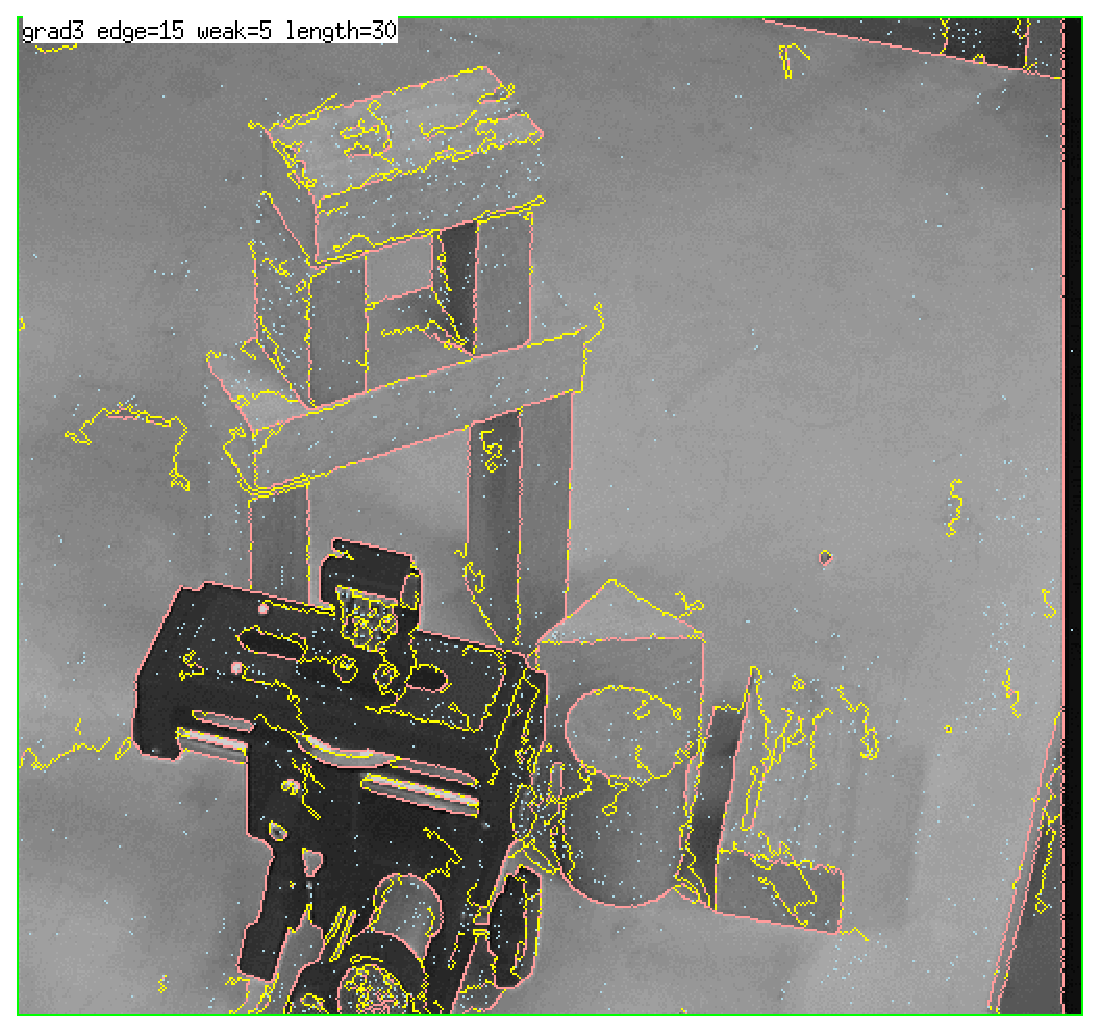
\includegraphics[height=9cm]{fig/block1.edg.ps}
%\epsfile{file=fig/block1.edg.ps,height=9cm}
\caption{Edge Finder and Overlaid Edges}
\end{center}
\end{figure}
\subsection{\label{tracking}Tracking}
{\tt "vision/correlation"} defines functions to find
correlation between window-image and tracking-image.

\begin{refdesc}
\classdesc{tracking-window}{pixel-image}{x-pos y-pos x-vel y-vel\\
\>pattern-size window-size\\
\>x-win y-win window window-margin\\
\>update threshold half-pattern correlation}{
This class defines tracking window.}

\methoddesc{:correlation}{}{
returns correlation between window-image and this image.}
\methoddesc{:grab}{\&optional (x x-pos) (y y-pos) (sampling 2)}{
grabs video image and returns grabbed pixel-image.}
\methoddesc{:window-rectangle}{val}{
draws rectangle on xwindow.}
\methoddesc{:rectangle}{val}{
draws rectangle on xwindow.}
\methoddesc{:move}{newpos \&aux (newx (aref newpos 0)) (newy (aref newpos 1))}{
moves tracking-window to {\em newpos} and grabs video image.}
\methoddesc{:track}{display-window \&optional th}{
tracks this image from window image.}
\methoddesc{:search}{display-window \&optional th}{
searches this image from window image.}
\methoddesc{:track-and-search}{flag \&optional th}{
tracks this image. If mistake tracking, searches this image from window image.}

\methoddesc{:pos}{}{
returns up-left position of window.}
\methoddesc{:vel}{}{
returns tracking velocity.}
\methoddesc{:insidep}{pos \&aux (x (aref pos 0)) (y (aref pos 1))}{
checks {\em pos} that is contained with tracking window.}
\methoddesc{:update}{\&optional (flag :get)}{
sets {\em flag} as update. if flag doesn't exist, returns update.}
\methoddesc{:prin1}{strm \&rest mesg}{
prints this tracking-window object with its name and dimensions.}
\methoddesc{:init}{x y size win-size}{
creates tracking-window object and sets slots.}
\end{refdesc}

\subsection{\label{PBMfile}Image File I/O}
%There are lots of file formats defined for the representation of
%pixel images.
{\tt "vision/pbmfile"} defines functions to transfer
image data between EusLisp and disk files.
EusLisp can read and write pgm
(portable gray-scale map) 
and ppm (portable pixmap) format files.

\begin{refdesc}
\funcdesc{read-pnm}{f \&optional buf0 buf1 buf2}{
reads a pgm or ppm file specified by file-stream {\em f} 
and returns a pixel-image or color-pixel-image object.
The image file can be either in ascii (P2 and P3) or in binary (P5 and P6) 
format.}
\funcdesc{read-pnm-file}{file \&optional buf0 buf1 buf2}{
reads a pgm or ppm file specified by filename {\em file}.}

\funcdesc{write-pgm}{f image  \&optional (depth 255)}{
writes a pixel-image specified by {\em image} into {\em f} file-stream
in the binary ppm format.
%(This function will be changed to allow adding comments.)
}
\funcdesc{write-ppm}{f image  \&optional (depth 255)}{
writes a pixel-image specified by {\em image} into {\em f} file-stream
in the binary pgm format.}
\funcdesc{write-pnm}{f img}{
writes a pixel-image specified by {\em img} into {\em f} file-stream.
If {\em img} is {\bf pixel-image}, it is written in the binary pgm format.
If {\em img} is {\bf color-pixel-image}, written in the binary
ppm format.}
\funcdesc{write-pnm-file}{file img}{
writes the pixel-image specified by {\em img} into {\em file}.
}
\funcdesc{image::read-raw-image}{file \&optional (x 256) (y x)}{
reads a raw-image file and returns a one-dimensional byte-vector (string).
%No assumption is made about the coordinates.
The dimensions of the raw-image must match with give {\em x} and {\em y}.
}
\funcdesc{image::write-raw-image}{file imgvec}{
writes pixel-values stored in a byte vector (string), {\em imgvec},
in {\em file}.}

\end{refdesc}


\subsection{JPEG compression/decompression}

EusLisp can link libjpeg.so in order to handle JPEG images.
Loading "eusjpeg.l" will define JPEG-compression and -decompression
functions.

